\section{Результаты и обсуждение}
% схему сюда. для того, чтобы решить поставленыеы задачи была прилумаоа соледующая схема эксперимента...

\begin{figure}[h]
    \begin{center}
        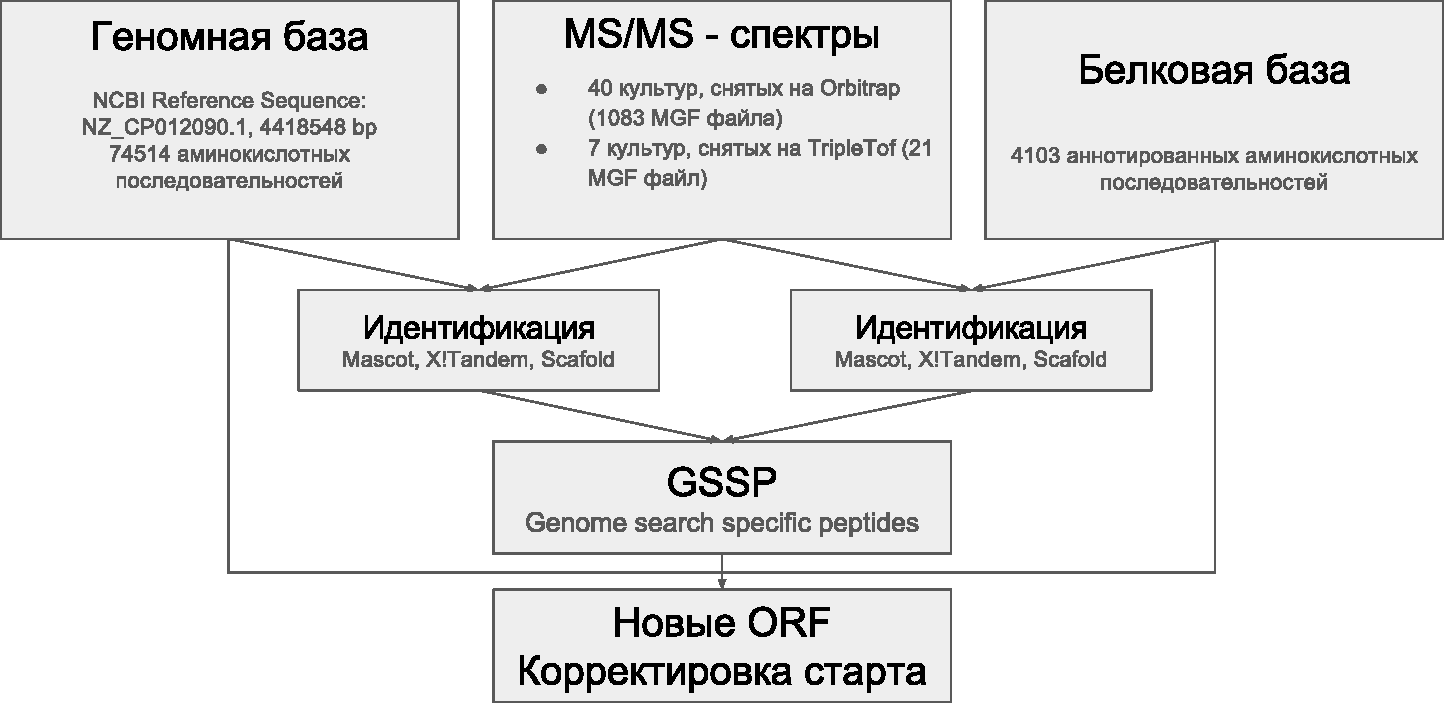
\includegraphics[width=1.\linewidth]{scheme.pdf}
    \end{center}
\caption[foo bar]{Схема анализа масс-спектрометрических данных. Можно выделить следующие ключевые шаги:
  \begin{enumerate*}%[label=\textit{\alph*)}]
    \item идентификация против белковой базы
    \item идентификация против геномной базы
    \item нахождение GSSP
    \item интерпретация GSSP
  \end{enumerate*}.}\label{scheme}
\end{figure}

Для решения поставленной задачи была разработана схема эксперимента, представленная на рисунке \ref{scheme}. Ключевыми этапами работы были идентификация против белковой и геномной базы, нахождение GSSP и их валидация, с последующей интепретацией.

\subsection{Подготовка и проведение масс-спектрометрических измерений}
%Тут что-нибудь про бактерий напиать.
Были отсняты масс-спектры 63 изолятов. Из них 6 были не фракционированы, остальные были разделены на 6 фракций. Разделение на фракции позволило идентифицировать пептиды, которые не были бы идентифицированы при обычном поиске, из-за того, что для измерения MS/MS спектра были бы отобраны более высоко представленные пептиды.
\subsection{Подготовка баз}
Скаченная из NCBI аннотация штамма W-148 содержала 4103 аннотированных белок-кодирующих последовательностей. После добавления контаминант и decoy-последовательностей получилась белковая база, состоящая из 8258 последовательностей. После транслирования генома в 6 рамках и исключения коротких последовательностей получилось 74488 белок-кодирующих последовательностей. В результате добавления контаминант и decoy-последовательностей, получилась геномная база, состоящая из 149028 последовательностей. Исключение коротких последовательностей из геномной базы позволило ускорить поиск; снизить пороговые значения идентификации, тем самым повысив чувствительность подхода. Минимальная длина аннотированного белка W-148 составляет 84 аминокислоты, таким образом, исключение рамок длинной менее 33 аминокислот не должно привести к потерям при идентификации.

\subsection{Идентификация белков и пептидов}
Поиск проходил при помощи поисковых машин Mascot и X!Tandem. Объединение результатов поиска и перерасчет FDR был произведен в Scaffold. На рисунке \ref{scaff_fdr} представлено распределение скорингов Mascot и X!Tandem. Черной сплошной линией обозначено пороговое значение, используемое Scaffold'ом. Пептиды, находящиеся правей и выше сплошной линии, считаются достоверно идентифицированными. Если бы использовался только Mascot, то достоверными считались бы пептиды, лежащие выше горизонтальной линии, а все, что ниже неё, считалось бы ложной идентификацией и не участвовало в дальнейшем анализе. С X!Tandem аналогичная ситуация, но пороговое значение обозначено вертикальной линией. Если бы бралось непосредственное объедение результатов двух поисковых машин, то достоверными считались бы пептиды из правой верхней области. Как видно, применение Scaffold позволяет значительно увеличить количество идентификаций. Это связано с тем, что в каждой поисковый машине реализованы свои поисковые алгоритмы, со своими характерными особенностями. Например, в Mascot не заложена возможность проверки того, что был отобран не моноизотопный ион, а у X!Tandem такой функционал имеет. Такая ситуация чаще всего возникает, если снимается спектр большого пептида. Если пептид короткий, то в нем мало атомов углерода (вероятность того, что среди 10 атомов углерода нет ни одного C13 примерно 90\%), соответственно большая часть пептидов будет иметь только атомы С12 и моноизотпный пик будет самым интенсивным. Если же пептид большой (вероятность, что среди 150 атомов углерода все С12 ~22\%, а вероятность того, что 149 атомов будут C12 и один C13 примерно 34\%), то моноизотпный пик будет иметь меньшую интенсивность, чем пик с одним С13. Другим ограничением Mascot является маленькое количество модификаций, которые могут быть одновременно заданы для поиска. Таким образом, не смотря на то, что Mascot является "золотым станадртом"\ при идентификации \cite{cox2011andromeda}, использование дополнительных поисковых инструментов позволяет значительно увеличить количество идентификаций и их качество. Результаты идентификации отснятых спектров для каждой культуры представлены в таблице \ref{tab_ident}.


\begin{figure}[h!]
    \begin{center}
        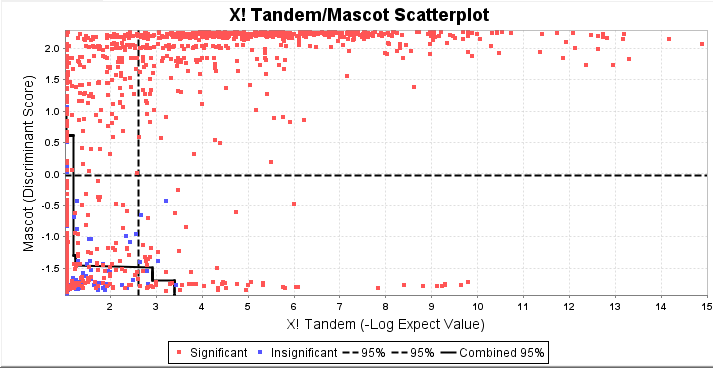
\includegraphics[width=0.9\linewidth]{scaff_fdr.png}
    \end{center}
\caption[foo bar]{Распределений скорнгов и количества идентификаций Macot (ось ординат), X!Tandem (ось абсцисс) и Scaffold. Красными точками обозначены достоверно идентифицированные пептиды, синими - обшибочно. Пунктирной линией обозначены пороговые значения для Macot и X!Tandem, соотвественно. Сплошной черной - итоговое пороговое значение, вычисленное Scaffold}
\label{scaff_fdr}
\end{figure}


\begin{longtable}{|P{3.5cm}|P{2cm}|P{2cm}|P{2cm}|P{2cm}|P{2cm}|}
\caption{Результаты идентификации. Применены следующие обозначения: protDB - белковая база; genDB - геноманя база; nPep - количество уникальных идентифицированных пептидов; nProt - количество уникальных идентифицированных белков; nGSSP - количество уникальных GSSP.} \label{tab_ident}
\hline 
\textbf{Культура}} & \textbf{protDB nPep} & \textbf{protDB nProt} & \textbf{genDB nPep} & \textbf{genDB nProt}} & \textbf{genDB nGSSP}\\ 
\hline 
\endfirsthead
\multicolumn{6}{c}%

{\tablename\ \thetable\ -- \textit{Продолжение прошлой страницы}} \\
\hline
\textbf{Культура}} & \textbf{protDB nPep} & \textbf{protDB nProt} & \textbf{genDB nPep} & \textbf{genDB nProt}} & \textbf{genDB nGSSP}\\ 
\hline
\endhead
\hline \multicolumn{6}{r}{\textit{Продолжение на следующей странице}} \\
\endfoot
\hline
\endlastfoot

Culture\_10140 & 6748 & 1425 & 6878 & 1431 &  19 \\ 
Culture\_10538 & 3290 & 893 & 3435 & 912 &   7 \\ 
Culture\_10540 & 3098 & 974 & 4252 & 1396 &  88 \\ 
Culture\_10785 & 6074 & 1489 & 6664 & 1619 &  71 \\ 
Culture\_1277 & 8500 & 1780 & 9111 & 1847 &  67 \\ 
Culture\_1604 & 7393 & 1688 & 8209 & 1794 &  81 \\ 
Culture\_19 & 8637 & 1796 & 9184 & 1837 &  43 \\ 
Culture\_1947 & 8709 & 1736 & 9216 & 1788 &  70 \\ 
Culture\_2093 & 9758 & 1913 & 10257 & 1946 &  57 \\ 
Culture\_2298 & 2365 & 999 & 2539 & 1025 &  12 \\ 
Culture\_23 & 4442 & 1229 & 5339 & 1433 &  57 \\ 
Culture\_243 & 5254 & 1468 & 6100 & 1589 &  66 \\ 
Culture\_2849 & 1248 & 613 & 1439 & 690 &  22 \\ 
Culture\_3123 & 928 & 472 & 1135 & 571 &  19 \\ 
Culture\_3325 & 2012 & 767 & 2279 & 827 &  20 \\ 
Culture\_333 & 4969 & 1365 & 5832 & 1535 &  65 \\ 
Culture\_3406 & 1396 & 524 & 1849 & 659 &  34 \\ 
Culture\_3432 & 6603 & 1591 & 7316 & 1657 &  50 \\ 
Culture\_3912 & 2064 & 687 & 2404 & 758 &  23 \\ 
Culture\_3984 & 2901 & 826 & 3364 & 940 &  24 \\ 
Culture\_4766 & 2579 & 867 & 3036 & 968 &  27 \\ 
Culture\_478 & 5906 & 1472 & 6444 & 1510 &  39 \\ 
Culture\_509 & 2756 & 1019 & 2963 & 1053 &  14 \\ 
Culture\_530 & 3339 & 1159 & 3544 & 1177 &  12 \\ 
Culture\_5583 & 5184 & 1365 & 5960 & 1503 &  50 \\ 
Culture\_5647 & 6794 & 1590 & 7493 & 1655 &  47 \\ 
Culture\_617 & 6408 & 1540 & 7070 & 1601 &  45 \\ 
Culture\_7283 & 9719 & 1889 & 10285 & 1930 &  62 \\ 
Culture\_7992 & 8311 & 1797 & 8765 & 1828 &  59 \\ 
Culture\_8009 & 4840 & 1141 & 4908 & 1173 &  18 \\ 
Culture\_8447 & 8624 & 1580 & 8570 & 1566 &  22 \\ 
Culture\_8836 & 5429 & 1259 & 5437 & 1247 &  16 \\ 
Culture\_9013 & 8002 & 1518 & 8028 & 1508 &  17 \\ 
Culture\_9207 & 3901 & 974 & 4011 & 985 &  10 \\ 
Culture\_9334 & 6287 & 1403 & 6371 & 1398 &  16 \\ 
Culture\_9412 & 1514 & 495 & 1640 & 514 &   7 \\ 
Culture\_9612 & 2709 & 568 & 2910 & 606 &   7 \\ 
Culture\_9622 & 6241 & 1540 & 6879 & 1640 &  54 \\ 
Culture\_9637 & 4125 & 1171 & 4327 & 1193 &   9 \\ 
Culture\_9859 & 1819 & 639 & 1915 & 646 &   5 \\ 
Culture\_K10140 & 5650 & 1211 & 5914 & 1227 &  23 \\ 
Culture\_K10538 & 2104 & 714 & 2224 & 754 &  14 \\ 
Culture\_K10785 & 4508 & 1239 & 5108 & 1317 &  30 \\ 
Culture\_K19 & 6124 & 1304 & 6464 & 1311 &  29 \\ 
Culture\_K23 & 2556 & 569 & 2714 & 585 &  14 \\ 
Culture\_K243 & 4008 & 1188 & 4293 & 1235 &  17 \\ 
Culture\_K2849 & 5615 & 1262 & 5917 & 1270 &  20 \\ 
Culture\_K3123 & 2572 & 567 & 2725 & 587 &  25 \\ 
Culture\_K3912 & 6484 & 1323 & 6780 & 1328 &  29 \\ 
Culture\_K3984 & 1372 & 393 & 1588 & 462 &  22 \\ 
Culture\_K509 & 4423 & 1304 & 4710 & 1340 &  22 \\ 
Culture\_K530 & 5695 & 1049 & 5905 & 1033 &  25 \\ 
Culture\_K8447 & 6115 & 1549 & 6455 & 1576 &  31 \\ 
Culture\_K9013 & 6428 & 1349 & 6796 & 1405 &  31 \\ 
Culture\_K9334 & 1836 & 548 & 2081 & 614 &  14 \\ 
Culture\_K9612 & 2276 & 695 & 2415 & 705 &  15 \\ 
Sp1 & 13934 & 1959 & 14914 & 2000 &  46 \\ 
Sp10 & 13056 & 2000 & 14368 & 2047 &  38 \\ 
Sp13 & 11230 & 1701 & 12974 & 1763 &  41 \\ 
Sp22 & 8674 & 1595 & 10687 & 1667 &  34 \\ 
Sp27 & 11972 & 1997 & 12872 & 2029 &  53 \\ 
Sp45 & 12996 & 2010 & 13958 & 2046 &  39 \\ 
Sp7 & 11933 & 1912 & 12790 & 1965 &  39 \\ 

\end{longtable}
		
Стоит отметить, что вычислительные мощности растут с каждым годом, при этом сложность протеомного поиска координально не меняется (современные приборы снимают больше спектров, что увеличивает сложность поиска, но при этом растет разрешающая способность, что сокращает поисковое пространство). Поиск образца в 10000 спектров против базы в 4000 последовательностей занимает чуть больше трех минут, и практически ничего не стоит (только разовая покупка лицензии, если программа платная). При этом время на подготовку образца и проведение эксперимента может достигать нескольких месяцев и требовать больших финансовых вложений. Это делает применение подходов с использованием нескольких поисковых машин ещё более привлекательным.  


В результате против белковой базы было идентифицировано 32054 пептида (1041059 psm), против геномной базы 36502 уникальных пептида (1131085 psm). Пересечение идентифицированных пептидов представлено на рисунке \ref{Identification}. Часть пептидов идентифицирована против белковой базы и не идентифицирована против более полной геномной базы. Это связано с различными пороговыми скорингами при поиске против баз разных размеров. 
После вычитания результатов поиска против белковой базы из результатов поиска против геномной базы получилось 6015 GSSP (Genome search specific peptides).  После исключения пептидов, представленных в аннотированном геноме и идентифицированных только против геномной базы, осталось 1397 GSSP. Наличие таких пептидов, идентифицируемых только против геномной базы и представленных в аннотации, связано с пересчетом FDR: при отдельном рассмотрении результатов идентификации каждой поисковой машины таких эффектов не возникает. После исключения GSSP, представленных только в одной культуре, осталось 425 пептидов. Результаты интерпретации GSSP при таких фильтрах: 16 новый ORF, и 304 гена с корректированным положением старта.  
Пептидов, интерпретируемых как пептиды перед аннотированным стартом примерно в 5.5 раз больше, чем пептидов, относящихся к новым генам. Такой разброс может быть связан с тем, что пептидам относящимся к корректировке рамки проще пройти порог FDR. В самом деле, при пептидном и белковом FDR в 1\% и, примерно, 1000000 psm при размере базы в 4000 аминокислотных последовательностей, 10000 пептидов будут ложно-положительно идентифицированы. Если брать критерий 2 и более пептидов для идентификации белка, то такого количества пептидов будет достаточно для идентификации 5000 белков, если не учитывать белковой FDR. С учетом белкового FDR количество ложно-положительно идентифицированных белков должно быть не боле 40. Для этого достаточно 80 пептидов. Таким образом, в экспериментах с большим количеством исходных данных, белковый FDR становится более жестким критерием, чем пептидный. Соответственно, GSSP относящимся к корректировке рамки проще пройти белковый FDR, так как в этой рамке так же присутствуют пептиды из аннотированной части последовательности. В случае нового гена в "прохождение"\ белкового FDR участвуют только GSSP пептиды.

\begin{figure}[ph!]
    \begin{center}
        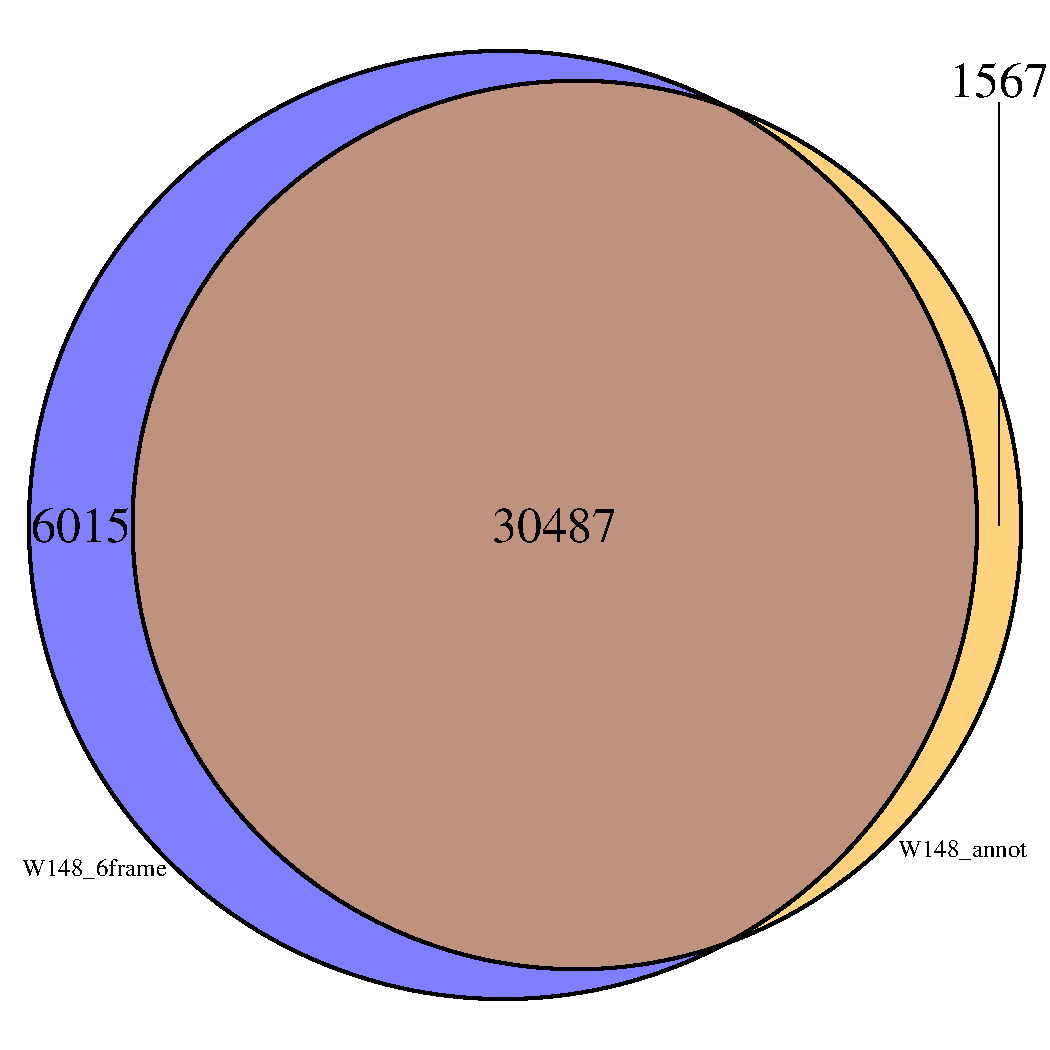
\includegraphics[width=0.9\linewidth]{Identification.pdf}
    \end{center}
\caption[foo bar]{Сравнение идентификаций против различных баз:
  \begin{enumerate*}%[label=\textit{\alph*)}]
    \item annot - количество уникальных пептидов идетифицированных против белковой базы
    \item 6frame - количество уникальных пептидов идетифицированных против геномной базы
  \end{enumerate*}.}
\label{Identification}
\end{figure}

Для подтверждения результатов были применены дополнительные критерии. После удаления PSM, ошибка идентификации которых составляет более трех стандартных отклонений в предположении о нормальном распределении ошибки идентификации всех PSM в интервале +/- 5 минут, остался 331 уникальный GSSP. Следует отметить, что на этом шаге отсекались пептиды, ошибка идентификации которых меньше, чем реальная точность приборов. Поэтому данный критерий отнесен к дополнительным. Затем была проведена фильтрация по времени выхода. После исключения 10\% наиболее отклоняющихся пептидов, остался 147 уникальный GSSP. На рисунке \ref{ret_time} изображено распределение калибровочных и GSSP PSM.

\begin{figure}[ph!]
    \begin{center}
        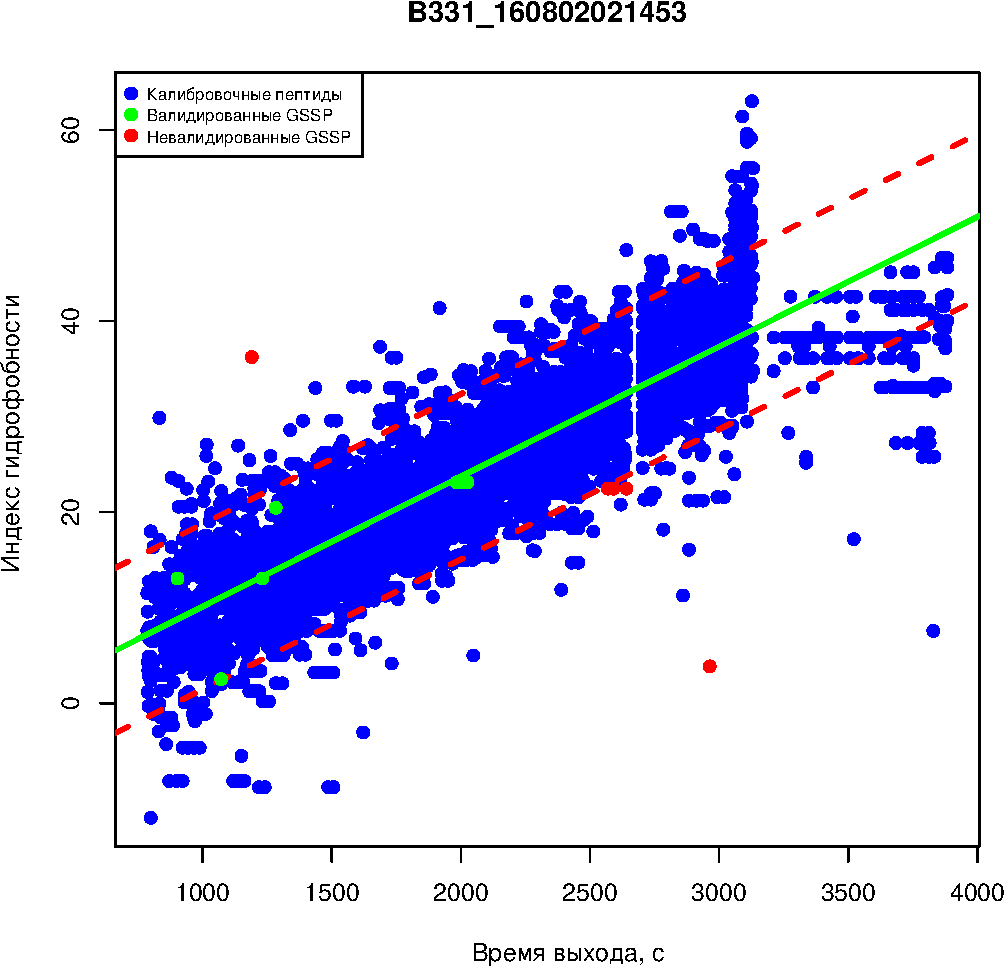
\includegraphics[width=1\linewidth]{ret_time.pdf}
    \end{center}
\caption[foo bar]{Распределение времени выхода из хроматографа и расчитаной величиной гидрофобности. Синим обозначены Калибровочные PSM, относящиеся к калибровочным пептидов. Зеленым и красным, PSM относящиеся к GSSP. Зеленой линией изображена регрессионая кривая, красной пунктирной - пределеные значения.}
\label{ret_time}
\end{figure}

Все GSSP были проверены на точное вхождение в базу NCBInr. Среди белков, в которых нашлись GSSP, не было найдено  таких, которые бы относились к организмам, которые ранее снимались на используемом масс-спектрометре. Таким образом, можно исключить остаточную контаминацию на приборе и пробоподготовке. Также были исключены 8 пептидов, которые присутствуют в аннотированной последовательности \ti{W-148} с учетом одной замены.

\subsection{Интерпретация новых событий}
\subsubsection{Новые ORF}
Было идентифицировано 16 новых ORF, в которых присутствует 2 и более уникальных GSSP. Из шестнадцати ORF пять пересекаются с аннотированными псевдогенами, одиннадцать лежат на комплиментарной цепи участков с аннотированными генами. У пяти из шестнадцати есть гомолог в H37Rv. Гены всех \ti{M. tuberculosis} плотно расположены, и межгенные области либо отсутствуют, либо их длинна намного меньше длины гена, либо, если межгенник большой, в нем находится псевдолен. Поэтому не найдено новых генов, которые не относились бы к псевдогенам и лежали в межгенном пространстве.

Следует отметить, что причины по которым ген становится "псевдогеном"\ с точки зрения биологии и системы аннотации NCBI различны. Так, наиболее частыми причинами из-за которых участок генома аннотируется как псевдоген являются: фреймшифт (потеря или вставка не кратного трем числа нуклеотидов, в результате чего нарушается белковая последовательность), неполный ген (присутствует только часть гена, в сравнении с гомологами), стоп-кодон по середине последовательности, низкое качество сборки (например, если ген находится на стыке контигов). Для всех идентифицированных псевдогенов была найдена "техническая"\ и "биологическая"\ причина, из-за которой они получили статус псевдогена. Пример идентифицированного псевдогена представлен на рисунке \ref{pseudo_1}.

\begin{figure}[ph!]
    \begin{center}
        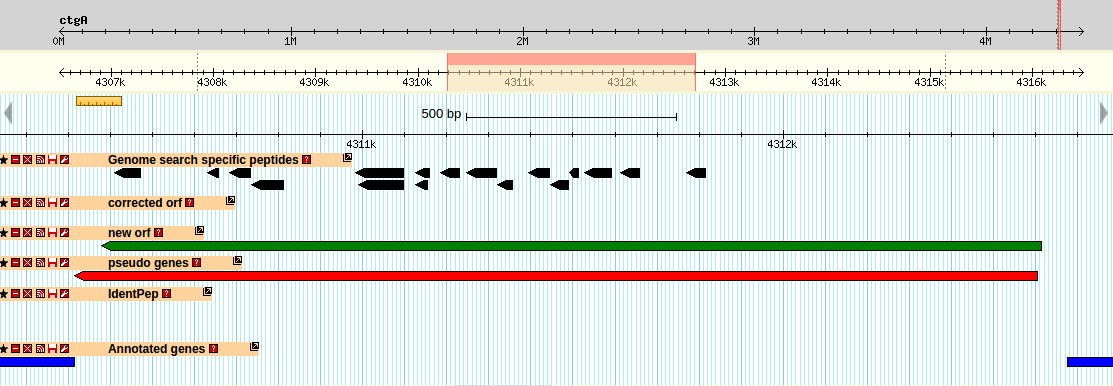
\includegraphics[width=1.2\linewidth, angle=-90]{pseudo_1.png}
    \end{center}
\caption[foo bar]{Идентифицированный псевдоген. Сними обозначены аннотированые гены, красным - псевдоген, зеленым - открытая рамка считывания, Genome search specific peptides - пептиды, идентифицируемы только про поиски против геномной базы}
\label{pseudo_1}
\end{figure}

\begin{figure}[ph!]
    \begin{center}
        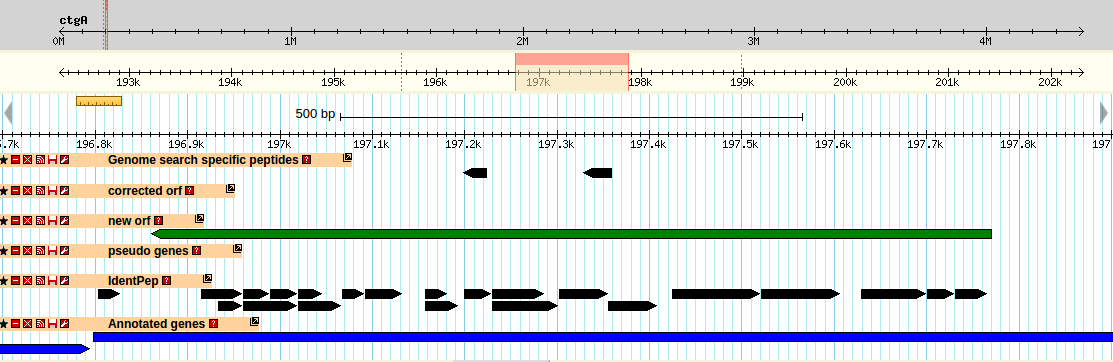
\includegraphics[width=1.2\linewidth, angle=-90]{comp_gene.png}
    \end{center}
\caption[foo bar]{ORF, лежащий на комплиментраной цепи к аннотированому и экспрессирующемуся гену. Сними обозначены аннотированые гены, IdentPep - идентифицрованные при поиске против белковой базы пептиды, красным - псевдоген, зеленым - открытая рамка считывания, Genome search specific peptides - пептиды, идентифицируемы только про поиски против геномной базы}
\label{comp_gene}
\end{figure}

\begin{figure}[ph!]
    \begin{center}
        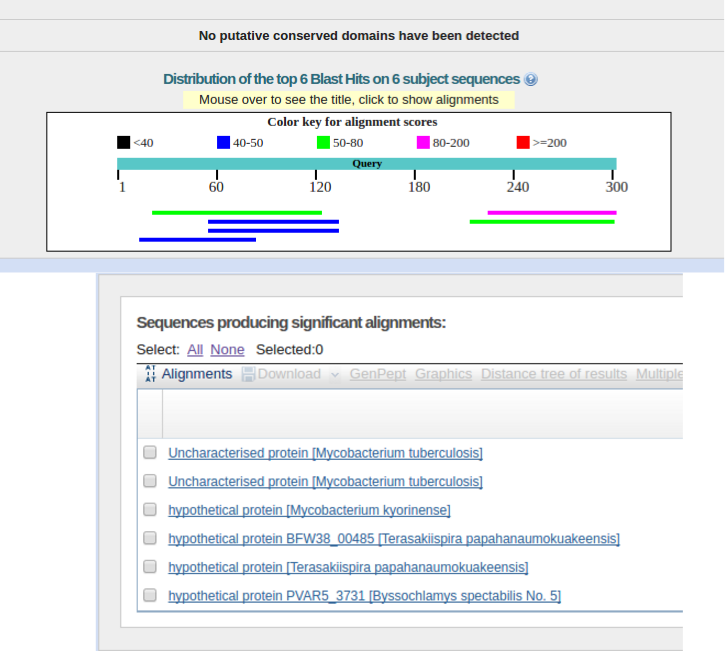
\includegraphics[width=1\linewidth]{comp_gene_blast.png}
    \end{center}
\caption[foo bar]{Результат поиска гомолога ORF, лежащей на комплиментарной цепи и предсталвенной на рисунке \ref{comp_gene}) против базы NCBInr с ипользованием алгоритма blast.}
\label{comp_gene_blast}
\end{figure}


В результате поиска против базы NCBInr при помощи алгоритма BLAST для десяти из одиннадцати ORF, лежащих на комплиментарной цепи (пример такого ORF представлен на рисунке \ref{comp_gene}) к аннотированным генам, были найдены гомологи. Эти гомологи были аннотированы как “гипотетический/предсказанный/непроверенный белок” другого штамма \ti{M. tuberculosis}. Косвенно результаты идентификации подтверждает тот факт, что все новые ORF лежат на комплиментарной цепи, а не в другом фрейме аннотированной. В самом деле, с пространственной точки зрения предположение, что транскрипт снимается с комплиментарной цепи выглядит более вероятным, чем предположение, что с одного транскрипта идет трансляция в двух фреймах двух разных аминокислотных последовательностей.

После применения дополнительных критериев фильтрации GSSP осталось шесть ORF с псевдогенами и один ORF на комплиментарной цепи.

\subsubsection{Корректировка положения аннотированного старта}
Всего 304 рамки содержат аннотированный ген и GSSP пептид. Распределение количества GSSP представлено на рисунке \ref{GSSP_stat}. Тот факт, что в большей части рамок нашелся только один GSSP может быть вызван двумя причинами. Либо, как отмечалось ранее, это ложно-положительно идентифицированные пептиды, прошедшие контроль FDR из-за большого количества  входных данных и наличия в рамке аннотированного гена. Либо, это может быть вызвано тем, что уже аннотированный старт находится близко к прошлому стоп-кодону, и на оставшемся участке ORF не может быть большого количества пептидов.
38 из 304 содержат два и более GSSP.  Эти рамки сравнили с гомологичными генами в H37Rv. 36 из 38 совпадают с точностью до SAP, 2 рамки длинней у W-148, чем у H37Rv. 

Не смотря на наличие нескольких тысяч аннотированных геномов \ti{M. tuberculosis}, валидация полученных результатов с помощью BLAST затруднительна, так как все штаммы аннотируются по гомологии. В результате получается множество аннотированных штаммов, аннотация которых зависит от H37Rv.



\begin{figure}[h!]
    \begin{center}
        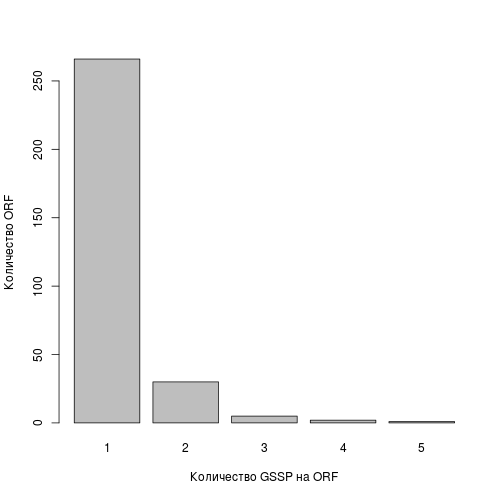
\includegraphics[width=1\linewidth]{GSSP_stat.png}
    \end{center}
\caption[foo bar]{распределения количества GSSP для корректировки рамки}
\label{GSSP_stat}
\end{figure}

\begin{figure}[h!]
    \begin{center}
        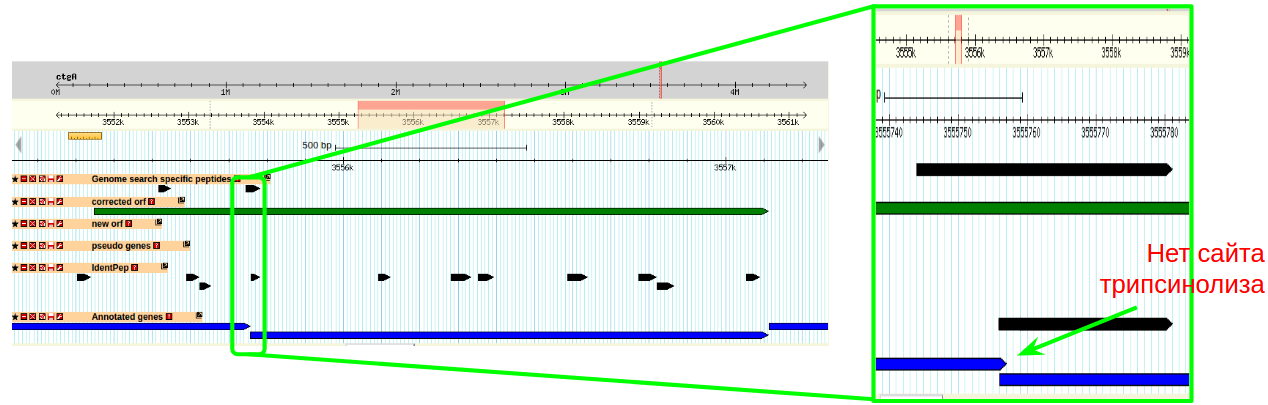
\includegraphics[width=1\linewidth]{overlap_pep.png}
    \end{center}
\caption[foo bar]{Ген с измененной рамкой считывания. Черным обозначены идентифицированные пептиды. Верхний глиф - GSSP, нижний - пептиды, идентифицированные при поиске против белковой базы. Идентифицирован как стартовый пептиды, так и overlap-пептид. Сайта трипсинолиза в этом месте нет}
\label{overlap_pep}
\end{figure}



\subsubsection{Пептиды, содержащие аннотированный старт}
Для 17 из 38 рамок, содержащих аннотированный ген и два более GSSP, были найдены пептиды, содержащие в себе стартовую аминокислоту для аннотированного гена. Такой пептид представлен на рисунке \ref{overlap_pep}. Для 7 из 38 были найдены пептиды, являющиеся стартовыми для аннотированного гена. У 3 из 38 найдены как стартовые, так и overlap-пептиды, причем в этом месте не было сайта трипсинолиза. Это может говорить об альтернативно сайте начала трансляции. В результате образуется две формы белка, причем одна является суффиксом другой. Существование генов с альтернативными сайтами начала трансляции показано в работе \cite{packham1997mammalian}. Для микобактерий такой результат был получен в работе Potgieter и коллег \cite{potgieter2016proteogenomic}, они нашли альтернативные старты для трех ORF.

\subsection{Программная часть}
В ходе работы было написано несколько десятков скриптов на языке R. Для работы с последовательностями использовались скрипты на Python 3. Ввиду того, что выдача поисковых программ стандартная, то полученный пайплайн можно легко перенести на любую другую бактерию. 
\newpage

